\chapter{Design and Implementation}


There are several goals and contributions I want to achieve. One main goal is to be able to recognize asbestos fibers in microscopic images, and show that transfer learning can be done even in this cross-domain specific task. Transfer learning is especially important, since there are only several hundred images to learn from. To achieve this, different CNN architectures are evaluated, with and without transfer learning. Also, in order to achieve better accuracy on the asbestos recognition task, I will alter the current architectures to better meet this specific task's characteristics. Data augmentation with several cropping methods and different combinations of the data set will be iterated over. As already mentioned in the introduction there is no baseline from the laboratory or any research that can be used for comparison. Therefore a new baseline needs to be established with a simple CNN. Also an inter-annotator agreement rate has been computed. In this chapter I explain and discuss the different methods used in this thesis, talk about modifications done on the architectures and dataset.

\section{Problem Description}

The provided dataset consists of about 2'000 microscopic images with and without asbestos fibers. The images come in two different dimensions and different qualities. Most of the images are 1024x768 pixels but some are in 1024x1024 pixels. Only a small subset was pre-labled and the remaining images needed to be labeled by hand, an error-prone task since I was never professionally instructed on how to do it. After labeling the images, some of them were sent back to the laboratory for checking the labeling, but there were many images, that the experts were uncertain on how to label and put them into a new folder which they called  "uncertain". From 441 images I labeled and sent the laboratory for checking 78 images came back as being suspected to contain asbestos but they were not quite sure. That's about 5.65\%. The detection of traces of asbestos by images is indeed very difficult and the error rate increases significantly as stated by the laboratory. In a next step these uncertain samples would be chemically examined to know for sure, which is beyond the scope of this thesis. In Figure \ref{fig:basic_examples} three example images are shown. One with asbestos, one without and one image with an error, that makes it difficult to be used for the training. The first dataset used includes all the images, but in later dataset alterations, these images with errors in them are removed.

\begin{figure}[t]
\centering
\subfigure{
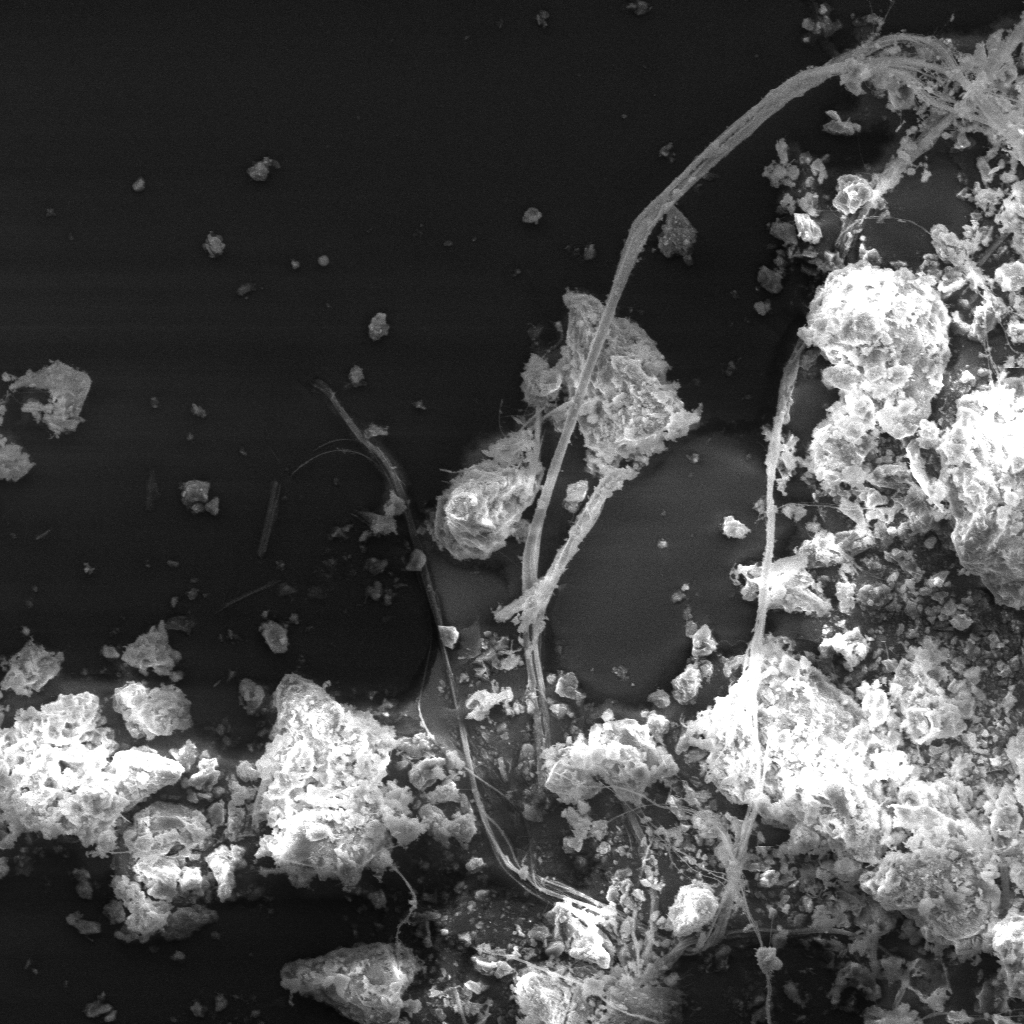
\includegraphics[width=.3\textwidth]{images/chapter4/asbestos.png}
}
\subfigure{
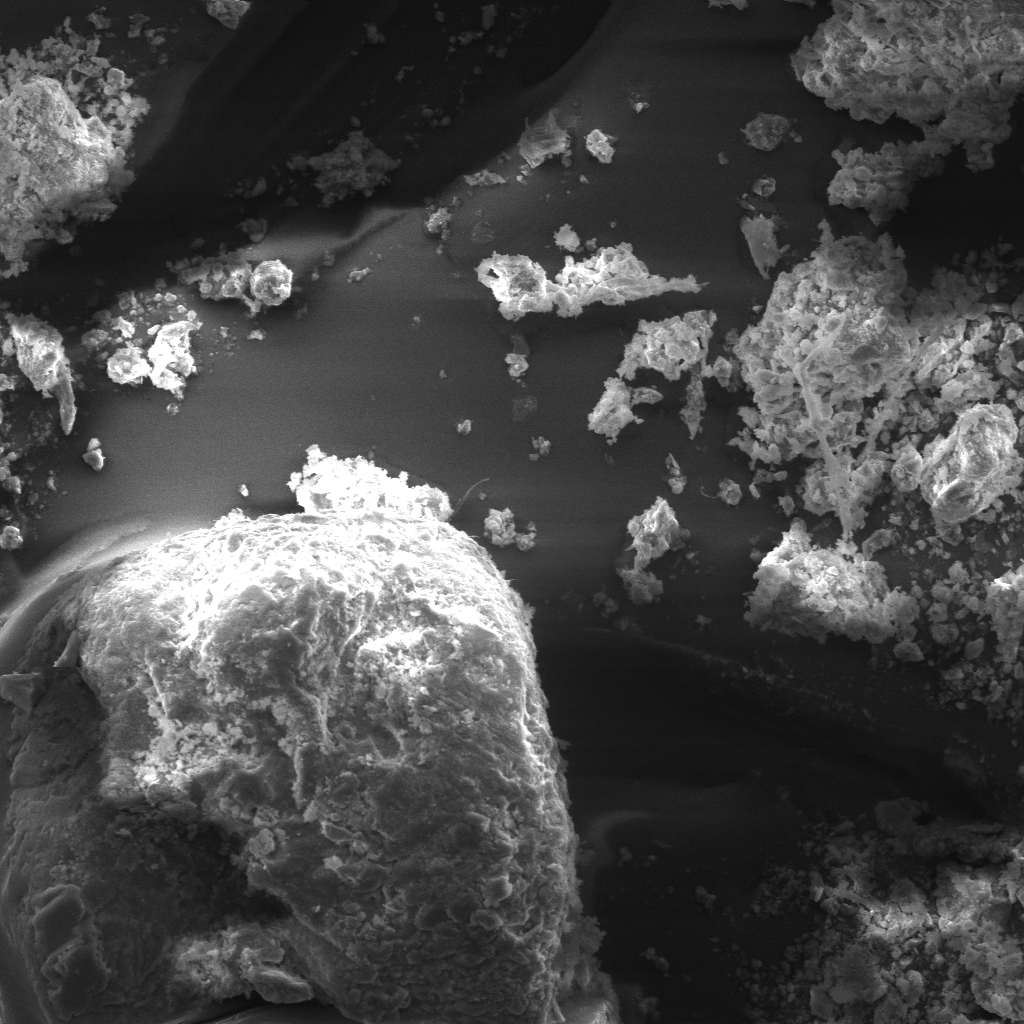
\includegraphics[width=.3\textwidth]{images/chapter4/non-asbestos.png}
}
\subfigure{
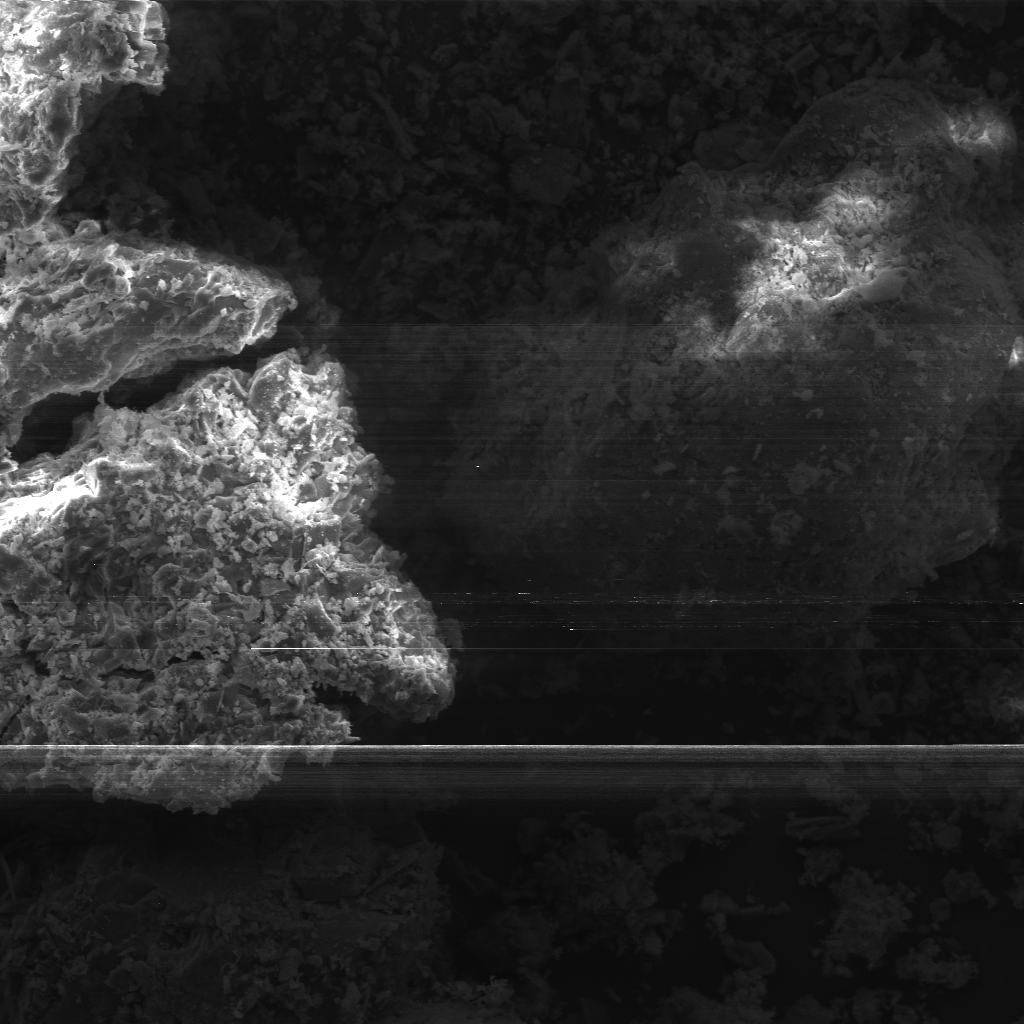
\includegraphics[width=.3\textwidth]{images/chapter4/fail.png}
}
\caption{On the left side the image shows a clear asbestos fiber, in the middle an image without asbestos is shown. On the right side, en example is provided of images that were processed with errors.}
\label{fig:basic_examples}
\end{figure}

Since the images are quite large, they will drastically increase in size, once decoded into a PIL object, or Tensor object. On the provided hardware, the memory of four Tesla K80 won't be enough to process whole images during training. Most architectures resize the images to much smaller dimensions ranging from 224x224 for ResNet to 299x299 pixels for Inception v3.

\section{Baseline}

There are two different methods used to acquire a baseline that can show improvements from changes in architectures and provide a better understanding of the data. The first one is to use a very basic CNN with grid search to find the best hyper parameters. This will give a first and low estimation of the accuracy that can be achieved. Also it provides a minimum requirement of this thesis, to improve on that performance. The other method is the inter-agreement rate or Randolphs' kappa which is a chance-adjusted measure of agreement for any number of classes and raters \cite{randolph2005free}. Randolphs' kappa is a free-marginal kappa that is used when the raters have no fixed number of cases assigned to a specific class as opposed to the traditional Fleiss' kappa, where raters know a priori how many elements a certain class expects. With the asbestos images, this is not the case and the raters have no knowlegde about the asbests versus non-asbestos ratio. Randolph's kappa is an extension of the Fleiss' kappa. For the calculation a online calculator is used \cite{humanlevel2014}.

\section{Data Augmentation}

One common problem in Deep Learning is the amount of data needed to be able to train a model well. This requirement of having huge datasets arises from the need to train an even larger number of parameters of the model, which usually goes into the millions for current state-of-the-art architecuters like VGG's \cite{simonyan2014very}, ResNet's \cite{he2016deep} or Inception \cite{szegedy2015going, szegedy2016rethinking}. Initially the weights for the filters are randomly chosen and then changed during backpropagation in order to lead to a lower loss from the loss function and hopefully lead to a higher generalizability. Having not enough images to train on will lead to a very poor inference through overfitting to the training images. Such a model will not generalize well to unseen data in the test-set even if the architecture has been trained until convergence. Convergence means having trained  for so many epochs, that there is no significant change in the weights from one epoch to another. Many studies have found some correlation between overall performance of the model and its size (number of parameters and layers) with lower layers of the model capturing very basic information like horizontal and vertical lines or color gradients whereas higher layers capturing the overall structure of the object that takes in more of the spatial characteristics. In order to mitigate the problem of overfitting more data is needed. There are only a few hundred good and usable images provided for the asbestos recognition task. They are highly specialized SEM images done in a very specific way including zoom, lightening and position. Finding more images on the internet is impossible so data augmentation is the only viable option to increase the dataset with more images to train on and therefore increase performance. A big dataset is required to be able to generalize the model and perform well on the test-set. Transfer learning might help but the fine-tuning still needs to be done after transferring the weights to the current task and more images allow better fine-tuning. Transfer learning and data augmentation are complementary methods to improve the performance.

Instead of working on the same set of images in every epoch, the images are randomly transformed in such a way, that the label still applies. Therefore every epoch learns with a new variation of the training-set thus reducing overfitting and creating much more images then there are present.

There two main forms of data augmentation. Offline and online augmentation. With offline data augmentation the images are augmented separately and saved to disk. This increases the overall size of the dataset by as many transformations that are done on an image. E.g. flipping horizontally and vertically would result in a three time increase of the dataset. The convolutional neural network would be able to more robustly classify objects in different places and different orientations leading to increased invariance. The downside of offline augmentation is the increase of disk space and therefore disk I/O during training that slows down the learning. With offline data augmentation the training process remains static and there is no randomness included. Adding more epochs would mean to learn more times on the same set of images present on disk.
Online data augmentation happens on the fly and does not need more disk space and disk I/O since it all happens in memory. The image is first loaded into memory and then several transformations are applied to the image. These transformations can be flipping, rotating, scaling, distorting and cropping in different places, and it all is done randomly. Especially the rotating and cropping when done randomly yields new images with every new epoch since the transformation is on a continuous scale. Online augmentation is therefore preferred since it leads to faster learning while reducing overfitting to the training images.

\section{Transfer Learning}

Finding millions of images on the internet of day-to-day objects is an easy task. Finding images on specialized objects like cancer cells in certain tissues is almost impossible. Especially when the equipment with all the settings is also different from hospital to hospital. To mitigate this problem transfer learning can be applied. With this method, the pre-learned weights for a certain architecture can be downloaded from the internet. These weights were obtained learning the model for a long time (until convergence) with a dataset like ImageNet. The hope is that the low and mid layer features are very similar even across problem domains. E.g. a cancer tumor has edges and colors (low-layer features) like any real world object from the ImageNet dataset and might even resemble certain real-life objects (mid-layer features). These layers can be used and fine-tuned to the current task. This gives the model a much better starting point other than initializing all weights of the model randomly and training them from scratch. 

It has been shown that pre-training on ImageNet indeed yields better results through obtaining good general-purpose features in tasks like image classification \cite{sharif2014cnn} and object detection \cite{girshick2014rich, sermanet2013overfeat}. But when the target domain is even farther away like for example human pose estimation \cite{carreira2016human}, image segmentation \cite{dai2016instance} and image captioning \cite{donahue2015long, karpathy2015deep}, pre-training on ImageNet seems to be able to help. Transfer learning has become the de facto standard for solving many different computer vision problems because it promises faster convergence and better accuracies despite the datasets getting bigger and the architectures deeper. Huh et al. \cite{huh2016makes} tried to shed light into this heuristic by examining how various aspects like number of classes, dataset size, ratio of  images per class and fine-grained versus coarse-grained class labels impact the performance of training from scratch versus fine-tuning with pre-trained weights. They found that although pre-training does help in many aspects the commonly held beliefes are not as accurate. For example they conclude that a significant reduction in number of classes or the number of images used in pre-training does not significatnly effect the performance of the transfer task, arguing that deep learning might not be as data-hungry as expected.

Generally the believe is that applying transfer learning can speed up the process of finding and developing good architectures.

This common knowledge that transfer learning always helps even across different target domains is not without critic. He et al. challenge this approach in a paper published in 2018 \cite{he2018rethinking}. They couldn't show that pre-training yielded better results on the COCO dataset than random initialization (training from scratch), only that it speeds up convergence very early in training. Better regularization and final target task accuracies were not obtained with pre-training. The main benefit of pre-training is that it converges faster and therefore training from scratch takes longer to catch up.
\\
They examined how various aspects like number of classes, dataset size and ratio of images per class impact the performance of training from scratch versus training with pre-trained weights. 

\section{AlexNext}

It has not been possible to get a baseline for the current performance or even an accurate estimation of human performance in the detection of asbestos fibers in the provided images. Therefore, AlexNet was used to create a baseline on which improvements may be observed and would allow discussions on architectures and their performance. The hyper-parameters learning rate and learning rate decay have been optimized with grid search as shown in Table \ref{tbl:similarity-test-map}. The model has been run for 50 epochs, although convergence has been observed much earlier as seen in Figure XXX.

\begin{table}[t] \centering
\ra{1.3}
\caption{AlexNet accuracies for baseline with optimized hyper-parameters}
\begin{tabular}{@{}rrrr@{}}
\toprule & learning rate & lr-decay & accuracy \\
\midrule
AlexNet        & 0.1         & 5        & 52.18\%  \\
AlexNet        & 0.05         & 5        & 53.64\%  \\
AlexNet        & 0.01         & 5        & 53.37\%  \\
AlexNet        & 0.005         & 5        & 53.67\%  \\
AlexNet        & 0.001         & 5        & 78.82\%  \\
AlexNet        & 0.0005         & 5        & 78.55\%  \\
AlexNet        & 0.0001         & 5        & 77.09\%  \\
\bottomrule
\end{tabular}
\label{tbl:AlexNetBaseline}
\end{table}


\section{Inception / ResNet}

Talk about other architectures and why they are important

\section{SigOpt Optimization}

What is SigOpt and why did I use it?

\section{Visualization}

Talk about different visualizations and what kind of visualizations make sense for this problem, what can be deduced from it and so on... 

\section{Different Dataset Variations}

The dataset plays an important role in the asbestos recognition task, partly because the dataset is very small and having some miss-classifications in the train set might lead to poor performance. Also with different cropping techniques it might get useful to reduce the size of the training by removing certain images. As will be explained in the next section cropping an image might invalidate the label, therefore making learning almost impossible. The original dataset is called FINAL and consists of all the provided images from the laboratory reduced by images that have obvious quality flaws in them as shown in Figure  \ref{fig:basic_examples}. In all subsets only the training folder has been altered, by adding or removing images. The test set has never been touched and remains the same for all the variations. The first subset of the FINAL dataset is the FINAL\_C dataset. Very unclear or questionable images have been removed from the training folder. In the FINAL\_CH dataset even more images have been removed from the training data, especially asbestos images that have a high chance of being cropped in a way, that there won't be any asbestos in the crops at all. E.g. if an image has an asbestos fiber in the very far corner of the image and nowhere else, it most likely won't be cropped that the label is preserved correctly. The next subset is FINAL\_C\_B which is similar to the FINAL\_C dataset but non-asbestos images have been uniformely removed in order to roughly match the asbestos images in numbers. The FINAL\_CH\_B datset is similar to the FINAL\_CH dataset but again balanced. The last dataset variation is FINAL\_EXTENDED where the validation images have been copied to the training. Evaluation looses it's purpose but the training data is extended by almost 20\% which could possibly lead to better results. That is feasible since the dataset is very small and could benefit from having more images. Table \ref{fig:cnn-basic-baseline} summarizes the datasets and their number of images.

\begin{table*}[h]
    \ra{1.3}
    \caption{Accuracy (\%) for several learning rates and lr-decays for CNN\_Basic as a baseline.}
    \centering
    \begin{small}
    \textsc{
      \resizebox{0.99\textwidth}{!}{%
      \begin{tabular}{rcclcclcc}
      \toprule 
      & \multicolumn{2}{c}{Train Set} && %
        \multicolumn{2}{c}{Validation Set} && %
        \multicolumn{2}{c}{Test Set} \\
      \cmidrule{2-3} \cmidrule{5-6}  \cmidrule{8-9}
      & asbestos & non-asbestos  && %
        asbestos & non-asbestos  && %
        asbestos & non-asbestos  \\ 
      \midrule
      FINAL                           & 485 & 721 && 152 & 227 &&  122 & 181 \\
      \midrule
      FINAL\_C                      & 438 & 672 && 152 & 227 &&  122 & 181 \\
      FINAL\_C\_B                  & 438 & 570 && 152 & 227 &&  122 & 181 \\
      \midrule
      FINAL\_CH                  & 359 & 672 && 152 & 227 &&  122 & 181 \\
      FINAL\_CH\_B              & 359 & 570 && 152 & 227 &&  122 & 181 \\
      \midrule
      FINAL\_EXTENDED        & 636 & 947 && 152 & 227 &&  122 & 181 \\
    \bottomrule
    \end{tabular}}
    }
    \end{small}
    %\end{center}
    \vspace{-3.9mm}
    \label{tbl:cnn-basic-baseline}
\end{table*}

\section{Cropping}

Talk about FiveCrop and RandomNine

\section{ResNet18 alterations}

Talk extensively about my new architectures where I try to increase the input image. I actually achieved best results with the old dataset of around 93\% accuracy with going down with the filters.... so from some million parameters I went  down to only 40'000 parameters and achieved best results... I will have to go into this much more